\documentclass[8pt, letterpaper]{report}

% Paquetes --------------------------------------------------------------------------
\usepackage{bm}
\usepackage{setspace}
\usepackage{titlesec}
\usepackage[colorlinks=true,linkcolor=blue,citecolor=blue,urlcolor=blue]{hyperref}
\usepackage{fancyhdr}
\usepackage{array}
\usepackage{amsfonts}
\usepackage{mathtools}
\usepackage{float}
\usepackage{caption}
\usepackage{fixmath}
%\captionsetup[figure]{name=Figura}
\counterwithout{figure}{chapter}
\counterwithout{table}{chapter}
\usepackage{tocloft}
\usepackage{amssymb,amsmath,amsthm} % Símbolos matemáticos
\usepackage[spanish]{babel} % Idioma
\usepackage[table,xcdraw]{xcolor}
\usepackage[utf8]{inputenc} % Acentos y otros símbolos 
\usepackage{enumerate} % Páginas
\usepackage{graphicx}
\usepackage{multirow}
\usepackage{physics}
\usepackage{subcaption}
\usepackage{multicol}
\usepackage{siunitx}
\usepackage{color}
\usepackage{braket}
\usepackage[nottoc]{tocbibind}
%\usepackage{natbib}
%\usepackage[square,sort,comma,numbers]{natbib} %Para ver solo números
%\usepackage[square,sort,comma]{natbib}
\usepackage[style=ieee, backend=biber, maxnames=2]{biblatex}
\addbibresource{PropuestadeTesis.bib}
\setlength{\parindent}{0pt} %Quitar indentación
\decimalpoint

%Definiciones paras las ecuaciones y las figuras --------------------------------------

% Redefinir el comando \theequation para incluir el número de sección y subsección
\renewcommand{\theequation}{\thechapter.\arabic{equation}}

\DeclareCaptionFormat{myformat}{\textbf{#1#2} #3}
\captionsetup[figure]{format=myformat}

\addto\captionsspanish{\renewcommand*\contentsname{Tabla de contenido}}
\addto\captionsspanish{\renewcommand*\listtablename{Lista de tablas}}
\addto\captionsspanish{\renewcommand*\tablename{Tabla}}
\addto\captionsspanish{\renewcommand*\listfigurename{Lista de figuras}}

\renewcommand{\cftfigpresnum}{Figura }
\setlength{\cftfignumwidth}{5em}
\renewcommand{\cfttabpresnum}{Tabla }
\setlength{\cfttabnumwidth}{5em}

\tocloftpagestyle{fancy}
\setlength\cftbeforetoctitleskip{1cm}
\setlength\cftbeforeloftitleskip{1cm}
\setlength\cftbeforelottitleskip{1cm}


% Reiniciar el contador de ecuaciones al principio de cada subsección -------------------------

\makeatletter
\@addtoreset{equation}{section}
\makeatother

% Configuración de márgenes
\usepackage[left=3cm, right=2.5cm, top=3cm, bottom=3cm]{geometry}

% Configuración del interlineado
\renewcommand{\baselinestretch}{1.5}

% Configuración de títulos de secciones
\titleformat{\chapter}[display]
  {\normalfont\huge\bfseries}{\chaptertitlename\ \thechapter}{20pt}{\Huge}
\titlespacing*{\chapter}{0pt}{-50pt}{40pt}

% Título de la tesis
\title{Ecuaciones de Estado de Estrellas de Neutrones mediante la Teoría Relativista de Campo Medio}
\author{Nicolas Mantilla Molina}
%\date{Fecha}

% Configuración de puntos en la tabla de contenidos
\renewcommand{\cftchapleader}{\cftdotfill{\cftsecdotsep}}
\renewcommand{\cftchapdotsep}{\cftdotsep}

% Configuración de encabezado y pie de página
\pagestyle{fancy}
\fancyhf{} % Limpia los encabezados y pies de página predeterminados
\fancyhead[L]{\leftmark}
\fancyhead[R]{\thepage}

% Redefinir el estilo de página de la primera página de cada capítulo
\fancypagestyle{plain}{%
  \fancyhf{} % Limpia los encabezados y pies de página predeterminados
  \fancyhead[L]{}
  \fancyhead[C]{Universidad Industrial de Santander}
  \fancyhead[R]{\thepage}
}
\titlespacing*{\chapter}{0pt}{50pt}{20pt} %Cambio los valores del espacio entre el título del cap y el encabezado

\begin{document}

% Portada
\begin{titlepage}
    \centering
    %\begin{minipage}[b]{0.45\textwidth}
    %    \includegraphics[width=\textwidth]{Figuras/logouis.png}\par\vspace{1cm}
    %\end{minipage}
    %\hfill
    %\begin{minipage}[b]{0.45\textwidth}
    %    \includegraphics[width=\textwidth]{Figuras/loGOTS.png}\par\vspace{1cm}
    %\end{minipage}
    \vspace{5cm}
    \rule{\textwidth}{2pt}
    {\LARGE\bfseries ECUACIONES DE ESTADO DE ESTRELLAS DE NEUTRONES MEDIANTE LA TEORÍA RELATIVISTA DE CAMPO MEDIO\par}
    \rule{\textwidth}{2pt}
    \vfill
    {\Large\itshape Nicolas Mantilla Molina\par}
    \vspace{1cm}
    {\Large\itshape Trabajo de grado para optar por el título de:  \\
    \textbf{Físico} \par}
    
    \vspace{.8 cm}
    {\Large\itshape Directora: \par}
    {\Large\itshape Laura Marcela Becerra Bayona, PhD \par}
    %\vfill
    \vspace{0.5cm}
    {\Large\itshape Co-directores: \par}
    {\Large\itshape José Fernando Rodriguez Ruiz, PhD \par}
     {\Large\itshape Luis Alberto Núñez de Villavicencio, PhD \par}
    \vfill
    %\vspace{.8cm}
    {\scshape\Large Universidad  Industrial De Santander \par}
    {\scshape\Large Facultad de Ciencias \par}
    {\scshape\Large Escuela de Física \par}
    {\scshape\Large Bucaramanga \par}
    {\scshape\Large 2025 \par}
\end{titlepage}


% Dedicatoria
\clearpage
\thispagestyle{empty}
\vspace*{\fill}
\begin{flushright}
    {\Large\itshape Dedicatoria\par}
    \vspace{0.5cm}
	Cuerpo de la dediatoria
    
\end{flushright}
\vspace*{\fill}
\clearpage

% Agradecimientos
\clearpage
\thispagestyle{empty}
\vspace*{\fill}
\begin{flushleft}
    {\huge\bfseries Agradecimientos\par}
    \vspace{0.5cm}
	Cuerpo de los agradecimientos
    
\end{flushleft}
\vspace*{\fill}
\clearpage



% Tabla de contenido
\pagestyle{empty}
\tableofcontents


% Lista de figuras
\clearpage
\listoffigures
\clearpage

% Página de resumen
\clearpage
%\thispagestyle{empty}
\vspace*{1cm} % Ajusta este valor según tu preferencia
\begin{flushleft}
    {\huge\bfseries Resumen\par}
    \vspace{0.5cm}
    En el presente trabajo se propone obtener Ecuaciones de Estado (EdE) de una Estrella de Neutrones (EN) mediante la Teoría Relativista de Campo Medio (TRCM). Las EN son objetos cuyas condiciones extremas permiten estudiar la materia nuclear a altas densidades, inalcanzables en laboratorio con la tecnología actual. A través de las EdE, se busca modelar la relación entre  la presión y la densidad de energía en el núcleo estelar, lo cual resulta fundamental para describir propiedades observables de la EN como su masa,  radio y  deformación de marea. Este estudio responde a la necesidad de conectar modelos teóricos con datos experimentales y observacionales, especialmente  aquellos obtenidos por misiones como LIGO, VIRGO y NICER.
    
    Las EdE construidas contienen parámetros libres que describen las interacciones y propiedades microscópicas de la materia. Este proyecto tiene como objetivo construir y ajustar modelos de EdE utilizando datos astrofísicos recientes. Adicionalmente, se investigará la capacidad de la EdE hallada para predecir objetos en el Mass-Gap, un rango de valores entre estrellas de neutrones masivas y agujeros negros ligeros, cuya composición sigue siendo debatida. Este enfoque permitirá modelar la estructura de las EN y contribuir al conocimiento de la materia nuclear en condiciones extremas.

    
\end{flushleft}



% Añadir la página de resumen al PDF pero no a la tabla de contenidos
%\addcontentsline{toc}{chapter}{Resumen}


%Capítulo 1
\chapter{Introducción}
\thispagestyle{fancy}

% Introducción

La materia en las estrellas de neutrones (EN) alcanza uno de los estados más extremos y densos conocidos en el universo observable. Estos objetos compactos, resultado del colapso gravitacional de estrellas masivas (sugerido por primera vez en 1934 por Baade y Zwicky \cite{baadeRemarksSuperNovaeCosmic1934}), comprimen la materia a densidades que superan las condiciones terrestres \cite{glendenningCompactStarsNuclear2000}. Las propiedades y características de la materia nuclear a densidades tan altas son objeto de estudio en la actualidad. Estudiar estos objetos estelares abre las puertas a la comprensión de la materia densa, ofreciendo un laboratorio natural donde se pueden contrastar modelos teóricos mediante observaciones astrofísicas. En adición, es posible corroborar indirectamente la validez de teorías nucleares y subatómicas bajo condiciones actualmente inalcanzables en el laboratorio \cite{raaijmakersConstraintsDenseMatter2021}.

Para este trabajo, el estudio de las EN se centra en las Ecuaciones de Estado (EdE), que describen la relación entre presión, densidad de energía y temperatura, siendo clave para resolver las ecuaciones de Tolman-Oppenheimer-Volkoff (TOV). Estas ecuaciones determinan características macroscópicas de las EN, como la relación masa-radio y las propiedades de marea, que han sido objeto de observaciones cada vez más detalladas gracias a misiones como NICER \cite{romaniPSRJ09520607Fastest2022, fonsecaRefinedMassGeometric2021, antoniadisMassivePulsarCompact2013}, LIGO y VIRGO \cite{collaborationGWTC21DeepExtended2022,theligoscientificcollaborationGW170817ObservationGravitational2017, theligoscientificcollaborationGW190814GravitationalWaves2020}. Con estos avances, los modelos teóricos se ven enriquecidos y enfrentan desafíos, como la identificación de límites para la masa máxima de una EN posible en la naturaleza, o la existencia de una ``brecha de masa'' (Mass-Gap) entre las EN de mayor masa y los agujeros negros más ligeros \cite{shaoNeutronStarBlack2022a}.

En el desarrollo de EdE, la Teoría Relativista de Campo Medio (TRCM) surge como una teoría efectiva para modelar interacciones nucleares bajo condiciones extremas de densidad \cite{waleckaTheoryHighlyCondensed1974,waleckaRelativisticNuclearManyBody1986}. La TRCM permite construir EdE que consideran distintas composiciones y acoplamientos entre partículas, posibilitando ajustes a los modelos basados en observaciones y datos experimentales cercanos a la densidad de saturación nuclear \cite{dutraRelativisticMeanFieldHadronic2014}. Sin embargo, la estructura interna de las EN sugiere la posible presencia de fases exóticas de materia, tales como hiperones o materia de quarks, desafiando aún más las formulaciones de EdE, especialmente en aquellas estrellas que alcanzan masas cercanas a $2.5$ masas solares \cite{lopesNatureMassgapObject2022}. La búsqueda de una EdE que logre reproducir observaciones actuales es, por lo tanto, crucial no solo para describir el comportamiento de la materia nuclear densa, sino también para realizar estudios más detallados sobre el destino y evolución final de estos objetos.

En esta propuesta de investigación, se plantea construir modelos de EdE mediante la TRCM y ajustar sus parámetros a partir de las observaciones astrofísicas actuales. La exploración del espacio de parámetros contribuirá a identificar las implicaciones físicas de la materia en su forma más extrema según las observaciones y brindará predicciones de la teoría empleada sobre la naturaleza de los objetos ubicados en el Mass-Gap.

%Se plantea el problema de investigación a estudiar y se brinda un contexto más amplio en la sección \ref{Planteamiento}. A continuación, en la sección \ref{MarcoTeorico}, se expondrán los principales conceptos requeridos para abordar el problema de investigación. Los objetivos del trabajo se presentan en la sección \ref{Objetivos}, mientras que, en la sección \ref{Metodologia}, se presenta la metodología planteada para alcanzar los objetivos de investigación, así como el cronograma de actividades para el desarrollo del trabajo. 









 

%Capítulo 2
%\chapter{Macrofísica: Objetos Compactos}
%\thispagestyle{fancy}

% Marco teórico - Macrofísica


%\section{Relatividad General}


%\section{Solución de Schwarzschild}


%\section{Ecuaciones de Estructura}

%\section{Observaciones de Estrellas de Neutrones}

%masas, radios, etc.

\chapter{Macrofísica: Objetos Compactos}

Los objetos compactos representan uno de los laboratorios naturales más extremos del universo, en los que la materia alcanza densidades, presiones y energías extremas que permiten extender nuestra comprensión de la física fundamental. Las estrellas de neutrones, en particular, constituyen el resultado final del colapso gravitacional de estrellas masivas, comprimiendo la materia a densidades que alcanzan varios órdenes de magnitud por encima de la densidad nuclear, en entornos de presión y temperatura que son extremadamente difíciles de reproducir en laboratorios terrestres \cite{baadeSuperNovae1934}. El estudio de estos objetos requiere necesariamente del escenario de la Relatividad General de Einstein, donde la curvatura del espacio-tiempo responde al contenido energético del sistema y viceversa.

En este capítulo desarrollamos los fundamentos teóricos necesarios para describir la estructura y propiedades de las estrellas de neutrones desde una perspectiva macroscópica. Comenzamos con una revisión de los fundamentos de la Relatividad General, estableciendo las ecuaciones de campo de Einstein que gobiernan la dinámica del espacio-tiempo. Posteriormente, exploramos la forma general de geometrías esféricamente simétricas, que proporciona un modelo básico para comprender la estructura de los objetos compactos. A partir de estos fundamentos, derivamos las ecuaciones de estructura que relacionan las propiedades microscópicas de la materia con las características macroscópicas observables de las estrellas de neutrones. Todas las secciones anteriores están fundamentadas en base al texto de Misner et al. \cite{misnerGravitation2017}. Finalmente, presentamos una revisión de las observaciones astronómicas más relevantes que han refinado nuestro entendimiento de estos objetos en la última década.

\section{Relatividad General}

La teoría de la Relatividad General, formulada por Einstein en 1915 \cite{einsteinFeldgleichungenGravitation1915}, es la descripción más exitosa de la gravitación como manifestación de la curvatura del espacio-tiempo. Esta teoría establece que la presencia de materia y energía modifica la geometría del espacio-tiempo, y que esta curvatura, a su vez, determina el movimiento de la materia y la propagación de la energía. La Relatividad General se fundamenta en dos principios básicos: el principio de equivalencia, según el cual los efectos de un campo gravitacional uniforme son localmente indistinguibles de los efectos de una aceleración uniforme, permitiendo que la gravitación pueda ser ``eliminada'' localmente mediante la elección apropiada de un sistema de coordenadas en caída libre; y el principio de covariancia general, el cual exige que las leyes de la física tengan la misma forma en todos los sistemas de coordenadas, requiriendo que las ecuaciones de la teoría sean expresadas en términos de tensores para asegurar su invariancia bajo transformaciones generales de coordenadas. Una representación esquemática del principio de equivalencia puede verse en la figura \ref{fig:equivalence_principle}, donde la esfera roja aparentemente cae en ambos sistemas, uno es un cohete acelerado, el otro la superficie de la tierra, siendo los dos sistemas de referencia indistinguibles.

\begin{figure}[h]
	\centering
	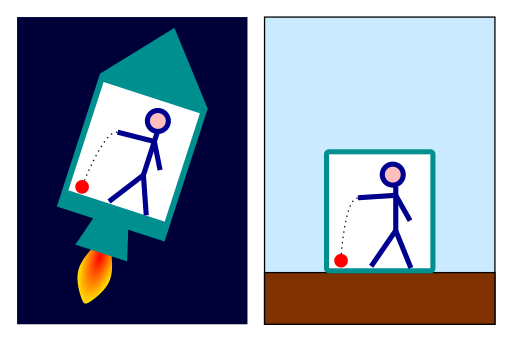
\includegraphics[width=0.7\linewidth]{Figuras/512px-Elevator_gravity.svg}
	\caption{Representación esquemática del principio de equivalencia. Markus Poessel.}
	\label{fig:equivalence_principle}
\end{figure}

\subsection{Ecuaciones de Campo de Einstein}

Las ecuaciones de campo de Einstein son un conjunto de ecuaciones diferenciales no lineales cuya forma compacta es:

\begin{equation}
	G_{\mu\nu} = 8\pi T_{\mu\nu},
	\label{eq:einstein_field}
\end{equation}

donde $G_{\mu\nu} = R_{\mu\nu} - \frac{1}{2}Rg_{\mu\nu}$ es el tensor de Einstein construido a partir del tensor de Ricci $R_{\mu\nu}$ y el escalar de curvatura $R$, y $T_{\mu\nu}$ es el tensor de energía-momento que describe las propiedades de la materia y energía presentes en el espacio-tiempo. Este conjunto de ecuaciones describe cómo la distribución de materia y energía determina la curvatura del espacio-tiempo, y cómo esta curvatura afecta el movimiento de la materia y la energía de vuelta. Las ecuaciones de Einstein satisfacen automáticamente las leyes de conservación del momentum y la energía a través de la identidad de Bianchi $G_{\mu\nu}{}^{;\rho} = 0$, lo que implica:

\begin{equation}
	\nabla_\rho T^{\mu\nu} = T^{\mu\nu}{}_{;\rho} = 0.
\end{equation}

Para describir la materia en el interior de las estrellas de neutrones, consideramos un modelo de fluido perfecto. El tensor de energía-momento es:

\begin{equation}
	T_{\mu\nu} = (\rho + P)u_\mu u_\nu - Pg_{\mu\nu},
	\label{eq:tensor_fluido_perfecto}
\end{equation}

donde $\rho$ es la densidad de energía del fluido, $P$ es la presión isótropa, y $u^\mu$ es la cuadrivelocidad del fluido, normalizada según $u^\mu u_\mu = 1$. Esta descripción asume que no hay flujos de calor, viscosidad, ni esfuerzos de corte en el fluido, aproximación válida para escalas de tiempo mucho mayores que los tiempos de relajación hidrodinámicos.

\section{Simetría Esférica}

Para describir la estructura de las estrellas de neutrones, vamos a resolver las ecuaciones de Einstein asumiendo simetría esférica y condiciones estáticas. La forma general de estas soluciones establece el punto de partida para entender tanto el interior como el exterior de objetos compactos con simetría esférica, en el marco de la teoría de la relatividad general. El elemento de línea de un sistema estático y esféricamente simétrico puede escribirse como:

\begin{equation}
	ds^2 = e^{2\phi(r)}dt^2 - e^{2\lambda(r)}dr^2 - r^2(d\theta^2 + \sin^2\theta d\varphi^2),
	\label{eq:metrica_esferica_general}
\end{equation}

donde $\phi(r)$ y $\lambda(r)$ son funciones arbitrarias de la coordenada radial $r$, y hemos utilizado coordenadas esféricas $(t,r,\theta,\varphi)$. La simetría esférica impone que la métrica sea invariante bajo rotaciones en el grupo $SO(3)$, mientras que la condición estática requiere la ausencia de términos cruzados $dt dr$, $dt d\theta$, y $dt d\varphi$, así como independencia explícita de la coordenada temporal. La métrica (\ref{eq:metrica_esferica_general}) representa la forma más general compatible con estas simetrías \cite{misnerGravitation2017}. Una representación gráfica de la geometría del espacio-tiempo que contiene una estrella con simetría esférica, estática, puede apreciarse en la figura \ref{fig:geometry-misner}, donde la región blanca representa la geometría exterior (fuera de la estrella), y la zona gris la región interior (dentro de la estrella).


%Para la métrica esféricamente simétrica (\ref{eq:metrica_esferica_general}), las componentes no triviales del tensor de Ricci son:
%
%\begin{align}
%	R_{tt} &= e^{2(\phi-\lambda)}\left[\phi'' + \phi'^2 - \phi'\lambda' + \frac{2\phi'}{r}\right], \\
%	R_{rr} &= -\phi'' - \phi'^2 + \phi'\lambda' + \frac{2\lambda'}{r}, \\
%	R_{\theta\theta} &= e^{-2\lambda}\left[r(\phi' - \lambda') - 1\right] + 1, \\
%	R_{\varphi\varphi} &= \sin^2\theta \cdot R_{\theta\theta},
%\end{align}
%
%donde $\phi' = \frac{d\phi(r)}{dr}$. Un resultado relevante para geometrías esféricamente simétricas es la posibilidad de expresar la función métrica $\lambda(r)$ en términos de una función de masa $m(r)$. Definiendo:
%
%\begin{equation}
%	e^{-2\lambda} = 1 - \frac{2m(r)}{r},
%	\label{eq:definicion_masa}
%\end{equation}
%
%la componente $R_{\theta\theta}$ del tensor de Ricci puede escribirse como:
%
%\begin{equation}
%	R_{\theta\theta} = r^2 e^{-2\lambda} \frac{1}{4\pi r^2}\frac{dm}{dr} - 1 + e^{-2\lambda}.
%\end{equation}

%Esta parametrización resulta especialmente útil porque la función $m(r)$ admite una interpretación física directa como la masa gravitacional contenida dentro de una esfera de radio $r$.

\begin{figure}[h]
	\centering
	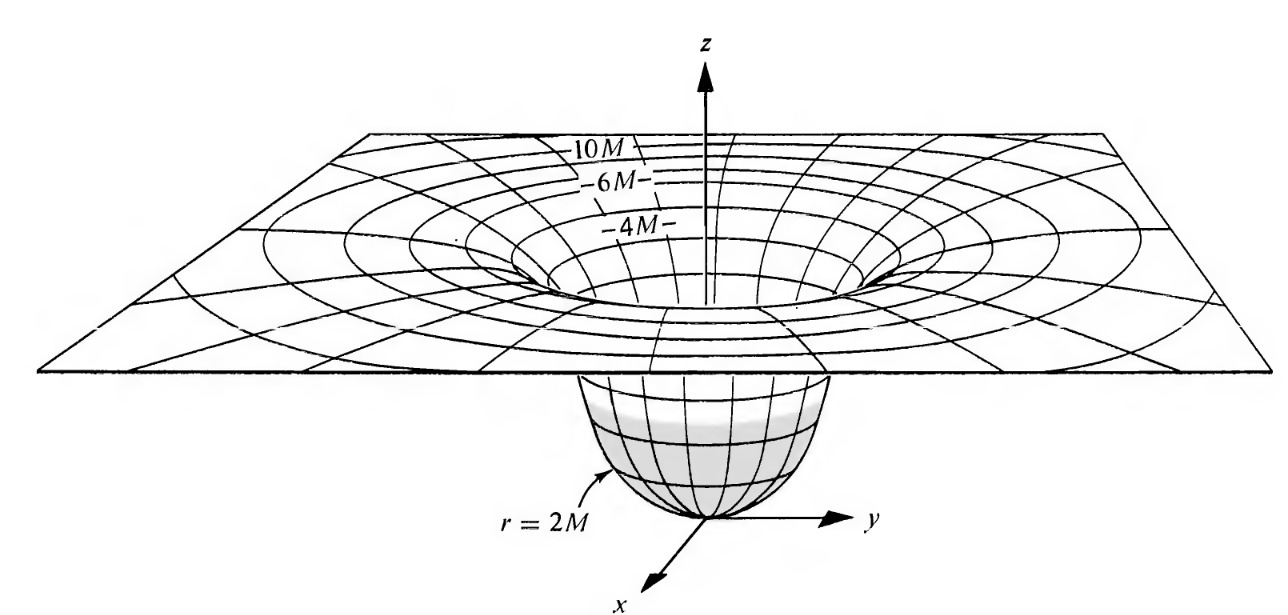
\includegraphics[width=0.7\linewidth]{Figuras/geometry-misner}
	\caption{Esquema de la geometría del espacio-tiempo de una estrella con simetría esférica. Tomado de \cite{misnerGravitation2017}.}
	\label{fig:geometry-misner}
\end{figure}

La solución general esférica (\ref{eq:metrica_esferica_general}) incluye varios casos de interés físico. En la región de vacío, cuando $T_{\mu\nu} = 0$, las ecuaciones de Einstein $G_{\mu\nu} = 0$ determinan completamente las funciones $\phi(r)$ y $\lambda(r)$, conduciendo a la solución exterior de Schwarzschild \cite{schwarzschildGravitationalFieldMass1999}. En el interior estelar, en presencia de materia con tensor de energía-momento (\ref{eq:tensor_fluido_perfecto}), las ecuaciones de Einstein proporcionan relaciones diferenciales entre $\phi(r)$, $\lambda(r)$, y las variables del fluido $\rho(r)$ y $P(r)$. En la superficie estelar, en $r = R$, las soluciones interior y exterior deben coincidir de manera continua, imponiendo condiciones de frontera específicas.

Para que la solución sea físicamente aceptable, las funciones métricas deben satisfacer condiciones de regularidad apropiadas. En el centro ($r = 0$) se requiere que $m(0) = 0$ y $\phi'(0) = 0$ para evitar posibles singularidades físicas o de coordenadas. En todo el espacio se debe cumplir que $e^{2\lambda} > 0$ y $e^{2\phi} > 0$ para mantener la signatura métrica consistentemente en el espacio-tiempo. En el infinito se exige que $\phi(\infty) = 0$ y $\lambda(\infty) = 0$ para recuperar la métrica de Minkowski, es decir, que en el infinito no haya influencia gravitacional de la estrella y el espacio-tiempo sea plano.

%Con la solución general esférica (\ref{eq:metrica_esferica_general}) y la parametrización de masa (\ref{eq:definicion_masa}) es posible derivar las ecuaciones de estructura que describen las propiedades al interior de las estrellas de neutrones y otros objetos compactos, como veremos en la siguiente sección.

\section{Ecuaciones de Estructura}

Las ecuaciones de estructura determinan la relación entre la distribución de materia en el interior de una estrella y la geometría del espacio-tiempo que genera. Para estrellas de neutrones, estas ecuaciones conectan las propiedades microscópicas de la materia densa con las características macroscópicas observables. En este sistema físico, el tensor de energía-momento del fluido perfecto (\ref{eq:tensor_fluido_perfecto}) actúa como fuente de las ecuaciones de Einstein (\ref{eq:einstein_field}). Las componentes del tensor de energía-momento en coordenadas esféricas son:

\begin{align}
	T_t^{\phantom{t}t} &= -\rho(r), \\
	T_r^{\phantom{r}r} &= T_\theta^{\phantom{\theta}\theta} = T_\varphi^{\phantom{\varphi}\varphi} = P(r).
\end{align}

Las ecuaciones de campo $G_{\mu\nu} = 8\pi T_{\mu\nu}$ establecen un sistema de ecuaciones diferenciales para las funciones métricas. Las componentes independientes son:

\begin{itemize}
	\item Componente $(t,t)$:
	\begin{equation}
		e^{-2\lambda}\left(\frac{2\lambda'}{r} - \frac{1}{r^2}\right) + \frac{1}{r^2} = 8\pi\rho.
		\label{eq:einstein_tt}
	\end{equation}
	\item Componente $(r,r)$:
	\begin{equation}
		e^{-2\lambda}\left(\frac{2\phi'}{r} + \frac{1}{r^2}\right) - \frac{1}{r^2} = 8\pi P.
		\label{eq:einstein_rr}
	\end{equation}
	\item Componente $(\theta,\theta)$:
	\begin{equation}
		e^{-2\lambda}\left[\phi'' + \phi'^2 - \phi'\lambda' + \frac{\phi' - \lambda'}{r}\right] = 8\pi P.
		\label{eq:einstein_theta}
	\end{equation}
\end{itemize}

Un resultado relevante para geometrías esféricamente simétricas es la posibilidad de expresar la función métrica $\lambda(r)$ en términos de una función de masa $m(r)$. Definiendo:

\begin{equation}
	e^{-2\lambda} = 1 - \frac{2m(r)}{r},
	\label{eq:definicion_masa}
\end{equation}

y utilizando esta parametrización en la ecuación (\ref{eq:einstein_tt}), obtenemos:

\begin{equation}
	\frac{dm}{dr} = 4\pi r^2 \rho(r),
	\label{eq:masa}
\end{equation}

donde la función $m(r)$ representa la masa gravitacional total contenida dentro de una esfera de radio $r$, y su interpretación física se hace clara al integrar la ecuación (\ref{eq:masa}):

\begin{equation*}
	m(r) = \int_0^r 4\pi r'^2 \rho(r') dr'.
\end{equation*}

De la ecuación (\ref{eq:einstein_rr}) y usando la parametrización (\ref{eq:definicion_masa}), la función métrica $\phi(r)$ satisface:

\begin{equation}
	\frac{d\phi}{dr} = \frac{m + 4\pi r^3 P}{r(r - 2m)}.
	\label{eq:phi}
\end{equation}

La ecuación (\ref{eq:phi}) determina la componente temporal de la métrica una vez conocidas las funciones $m(r)$ y $P(r)$. Finalmente, utilizando (\ref{eq:definicion_masa}), (\ref{eq:masa}) y (\ref{eq:phi}) para sustituir $\phi''$, $\phi'$ y $\lambda'$ de (\ref{eq:einstein_theta}), obtenemos la ecuación de equilibrio hidrostático relativista, también llamada ecuación de Tolman-Oppenheimer-Volkoff (TOV) \cite{oppenheimerMassiveNeutronCores1939}:

\begin{equation}
	\frac{dP}{dr} = -\frac{(\rho + P)(m + 4\pi r^3 P)}{r(r - 2m)}.
	\label{eq:tov}
\end{equation}

Esta importante ecuación describe el equilibrio entre la presión del fluido y la atracción gravitacional, incluyendo correcciones relativistas necesarias para sostener objetos compactos \cite{oppenheimerMassiveNeutronCores1939} y permitir su estabilidad. Para resolver el sistema de ecuaciones de estructura (\ref{eq:masa} - \ref{eq:tov}), se requiere de una ecuación de estado que relacione la presión y la densidad:

\begin{equation}
	P = P(\rho) \quad \text{o,} \quad \rho = \rho(P).
	\label{eq:ecuacion_estado}
\end{equation}

% Además, como condiciones de la estrella, se requiere tener una densidad central diferente de cero $\rho(0) = \rho_c > 0$ y se determina el limite exterior de la estrella $r = R$ como el punto donde la presión se anula $P(R) = 0$. En este punto, la masa total de la estrella es $M = m(R)$.

La solución se obtiene integrando numéricamente desde el centro hacia afuera, comenzando con una densidad central $\rho(0) = \rho_c > 0$ dada. El radio estelar $R$ se determina por la condición $P(R) = 0$, y la masa total $M = m(R)$ resulta de la integración de la ecuación de masa. En el límite no relativista ($M \ll R$ y $P \ll \rho$), la ecuación TOV se reduce a la ecuación clásica de equilibrio hidrostático:

\begin{equation}
	\frac{dP}{dr} = -\rho \frac{m}{r^2}.
\end{equation}

Para estrellas de neutrones, las correcciones relativistas en el sistema de ecuaciones son necesarias debido a su alta compacidad $M/R \sim 0.2-0.4$. Este sistema proporciona la base teórica para predecir las propiedades macroscópicas de las estrellas de neutrones a partir de modelos microscópicos de la materia nuclear densa.

\section{Observaciones de Estrellas de Neutrones}

Las observaciones astronómicas de estrellas de neutrones han experimentado una revolución en las últimas décadas \cite{pianMergersBinaryNeutron2021}, proporcionando restricciones cada vez más precisas sobre las propiedades de la materia densa. Estas mediciones permiten contrastar los modelos teóricos de ecuaciones de estado con la realidad física de estos objetos extremos. Las estrellas de neutrones se observan a través de múltiples canales electromagnéticos \cite{glendenningCompactStarsNuclear2000} y, recientemente, mediante ondas gravitacionales \cite{fonsecaNANOGravNineyearData2016}. Los principales métodos observacionales incluyen:

\begin{itemize}
	\item \textbf{Cronometraje de Pulsares}: Los pulsares son estrellas de neutrones altamente magnetizadas que emiten haces de radiación electromagnética. La precisión extrema en la medición de sus períodos de rotación permite determinar masas través del análisis orbital en sistemas binarios.
	
	\item \textbf{Astronomía de Rayos X}: Las estrellas de neutrones en sistemas binarios acretantes o como objetos aislados calientes pueden ser observadas en rayos X. Las misiones como NICER han revolucionado las mediciones de radio a través del modelado de puntos calientes superficiales.
	
	\item \textbf{Ondas Gravitacionales}: Las fusiones de estrellas de neutrones binarias, detectadas por LIGO-Virgo, proporcionan información sobre las propiedades de marea y la ecuación de estado a través de las modificaciones que introducen en la forma de onda gravitacional.
\end{itemize}

\subsection{Mediciones de Masa}

Las mediciones de masa de estrellas de neutrones se basan principalmente en el efecto Shapiro en sistemas binarios de pulsares. Este efecto relativista permite determinar las masas con alta precisión a partir del retraso temporal que experimenta la señal del pulsar al atravesar el campo gravitacional de su compañera.

Las mediciones más precisas incluyen:

\begin{itemize}
	\item \textbf{PSR J0740+6620}: Con una masa de $2.08 \pm 0.07 \, M_\odot$ \cite{fonsecaRefinedMassGeometric2021}, representa la medición más precisa de una estrella de neutrones masiva.
	
	\item \textbf{PSR J0348+0432}: Una estrella de neutrones con masa $2.01 \pm 0.04 \, M_\odot$ \cite{antoniadisMassivePulsarCompact2013}, crucial para establecer el límite inferior de la masa máxima.
	
	\item \textbf{PSR J0952-0607}: Con una masa reportada de $2.35 \pm 0.17 \, M_\odot$ \cite{romaniPSRJ09520607Fastest2022}, aunque con mayor incertidumbre debido al método de determinación basado en espectrofotometría.
\end{itemize}

Estas observaciones establecen que las estrellas de neutrones pueden alcanzar masas superiores a $2 M_\odot$, imponiendo restricciones sobre las ecuaciones de estado que deben ser suficientemente rígidas para soportar estas configuraciones. Otras estimaciones se han realizado empleando datos de ondas gravitacionales. Sin embargo, en mediciones mayores aún se discute la naturaleza del objeto observado (estrella de neutrones o agujero negro), como en el caso de GW190814 \cite{theligoscientificcollaborationGW190814GravitationalWaves2020} \cite{lopesNatureMassgapObject2022}, con una masa del objeto secundario estimado en $2.59^{+0.08}_{-0.09} M_\odot$.

\subsection{Mediciones de Radio}

La misión NICER (Neutron star Interior Composition ExploreR) ha proporcionado algunas de las primeras mediciones simultáneas de masa y radio para estrellas de neutrones específicas. Estas mediciones se basan en el modelado de puntos calientes en la superficie de pulsares de milisegundo, analizando las modulaciones en el flujo de rayos X.

Los resultados más significativos incluyen, a 1$\sigma$ de confiabilidad:

\begin{itemize}
	\item \textbf{PSR J0740+6620}: Análisis independientes con NICER y X-ray Multi-Mirror han proporcionado valores $R = 13.7^{+2.6}_{-1.5}$ km \cite{millerRadiusPSRJ0740+66202021} y $R = 12.39^{+1.30}_{-0.98}$ km \cite{rileyNICERViewMassive2021};
	
	\item \textbf{PSR J0030+0451}: $M = 1.44^{+0.15}_{-0.14} M_\odot$ y $R = 13.02^{+1.24}_{-1.06}$ km \cite{millerPSRJ0030+0451Mass2019};
	
	\item \textbf{PSR J0437-4715}: $M = 1.418 \pm 0.037 M_\odot$ y $R = 11.36^{+0.95}_{-0.63}$ km \cite{choudhuryNICERViewNearest2024}.
\end{itemize}

Adicionalmente, se han realizado estimaciones de radio mediante la medición del parámetro de deformación de marea en ondas gravitacionales \cite{kumarTheoreticalExperimentalConstraints2024}. Sin embargo, para obtener estas estimaciones es necesario realizar modelamiento adicional, lo que hace esta estimación modelo-dependiente. Para el caso de \textit{GW190814} y asumiendo el objeto secundario como una estrella de neutrones de rotación rápida, se estimó un radio ecuatorial de $R_e = 14.1^{+1.5}_{-2.0}$ km, mientras que asumiendo una estrella no rotante, se estimó un radio canónico de $R_{1.4} = 13.3^{+0.5}_{-0.6}$ km, ambos en el intervalo de confianza a 90 \% \cite{biswasGW190814PropertiesSecondary2021}.\\


Las observaciones combinadas de masa y radio imponen restricciones consistentes sobre las posibles ecuaciones de estado de la materia nuclear densa. Estas restricciones pueden resumirse como:

\begin{itemize}
	\item \textbf{Rigidez Suficiente}: La ecuación de estado debe ser lo suficientemente rígida para soportar masas $\geq 2 M_\odot$.
	
	\item \textbf{Radios Consistentes}: Los radios estelares deben estar en el rango $\sim 11-14$ km para masas típicas/canónicas de $\sim 1.4 M_\odot$.
\end{itemize}

Estas restricciones observacionales permiten restringir las posibles ecuaciones de estado de la materia nuclear densa. Al resolver el sistema de ecuaciones de estructura (\ref{eq:masa} - \ref{eq:tov}) junto con una ecuación de estado específica (\ref{eq:ecuacion_estado}), es posible predecir la masa y radio de las estrellas de neutrones a partir de modelos microscópicos. De esta manera, las observaciones astronómicas establecen el puente entre la física microscópica de la materia nuclear densa y las características macroscópicas observables de estos objetos compactos, guiando la construcción y validación de modelos teóricos.

\begin{figure}[h]
	\centering
	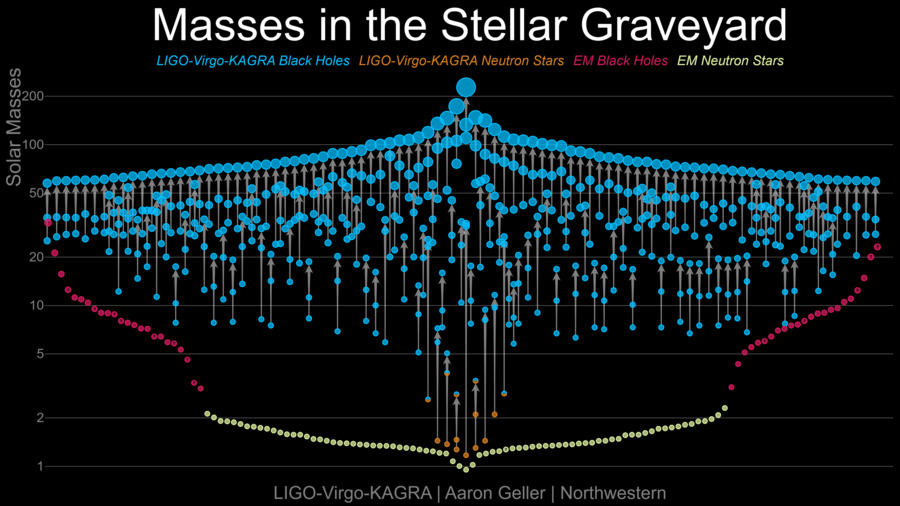
\includegraphics[width=0.7\linewidth]{Figuras/ligo-virgo-graveyard}
	\caption{Masas en el cementerio estelar. Contiene las masas estimadas mediante diferentes fuentes y su (posible) naturaleza, a enero de 2024. Tomado de \href{https://www.ligo.caltech.edu/image/ligo20250826d}{ligo.caltech.edu}.}
	\label{fig:ligo-virgo-graveyard}
\end{figure}

Las próximas generaciones de detectores de ondas gravitacionales, junto con misiones espaciales mejoradas y telescopios de nueva generación, prometen expandir significativamente nuestro conocimiento observacional de las estrellas de neutrones. Se espera que estas observaciones proporcionen restricciones aún más precisas sobre las ecuaciones de estado y posiblemente revelen nueva física en el régimen de densidades ultra-altas. Es claro que, a mayor número de observaciones, mayores son los requerimientos de nuestras teorías, lo que permite filtrar modelos físicos que pretendan describir la masa a densidades tan altas.
En particular, la detección de estrellas de neutrones con masas en el rango $2.5-3 M_\odot$ o la confirmación de transiciones de fase en el interior estelar a través de observaciones de estrellas, prometen descubrimientos de impacto para nuestra comprensión de la materia nuclear densa. En la figura \ref{fig:ligo-virgo-graveyard} se pueden apreciar las estimaciones de masa hasta enero de 2024, así como la posible naturaleza del objeto. Cabe destacar que en el rango de 2 a 5 M$_\odot$ hay incertidumbre en la naturaleza de varios objetos detectados.




%Capítulo 3
% Marco teórico - Microfísica
%\chapter{Microfísica: Ecuaciones de Estado}
%\thispagestyle{fancy}

% Introducción similar al capítulo sobre macrofísica. Aquí queremos mostrar brevemente la motivación de el estudio de ecuaciones de estado para entender la física de la materia en entornos tan densos y de tan alta energía.

%\section{Ecuaciones de Estado y Ejemplos}

%Definir las ecuaciones de estado (en este caso barótropas) y mostrar brevemente modelos y gráficas de modelos más simples: gas degenerado de neutrones, protones y electrones libres

%\section{Teoría Relativista de Campo Medio}

% Introducir la RMFT y mostrar las ventajas de una teoría relativista efectiva de campos mesónicos que se toman como uniformes mediante su valor medio en el estado base, frente a otros métodos como QCD y los Scrhodinger-based. Hablar sobre las simetrías y sus cantidades conservadas para explicar como se obtiene la expresión para la densidad de energía y de presión en una teoría de este estilo, construida sobre un lagrangeano.

%\section{Modelo del Estudio}

% Introducir el lagrangiano para un modelo que contenga neutrones, protones, electrones (campos esponoriales); un mesón escalar neutro sigma con autointeracciones de hasta 4to orden acoplado a la densidad escalar de nucleones, un mesón vectorial neutro omega acoplado a la corriente vectorial de nucleones y un mesón vectorial isovectorial neutro rho acoplado a la corriente de isospín de nucleones. Luego hallar las ecuaciones de movimiento para los campos, para finalmente llegar a la expresión de densidad de energía y presión. Hablar sobre los parámetros libres de este modelo.

%\subsection{Materia en Saturación Nuclear}

% Definir, explicar (importancia) y mostrar las mediciones de densidad de saturación, energía de enlace por nucleón, modulo de compresión, coeficiente de energía de simetría y pendiente del coeficiente de energía de simetría. Tomar las mismas mediciones de la propuesta.

\thispagestyle{fancy}
\chapter{Microfísica: Ecuaciones de Estado}

La descripción microscópica de la materia en entornos extremos de densidad es un problema de gran complejidad en la física moderna. En estas condiciones, con densidades que exceden significativamente la densidad nuclear de saturación, la materia exhibe comportamientos que requieren marcos teóricos que incorporen efectos relativistas y de muchos cuerpos. La ecuación de estado que gobierna esta materia establece la conexión directa entre la física microscópica de las interacciones nucleares y las propiedades macroscópicas observables de las estrellas de neutrones \cite{oppenheimerMassiveNeutronCores1939}.

La teoría relativista de campo medio surge como una herramienta particularmente adecuada para abordar este régimen, brindando un tratamiento consistente que respeta la causalidad mientras incorpora las interacciones nucleares fuertes \cite{glendenningCompactStarsNuclear2000}. Este formalismo permite extrapolar desde las propiedades conocidas de materia nuclear simétrica hacia las condiciones asimétricas y de alta densidad relevantes para objetos compactos.

\section{Ecuaciones de Estado y Ejemplos}

Una ecuación de estado define la relación termodinámica entre las variables que caracterizan el estado de equilibrio de un sistema físico. Para materia estelar a temperatura cero, consideramos ecuaciones de estado barotrópicas que relacionan la presión $P$ con la densidad de energía $\rho$ mediante (\ref{eq:ecuacion_estado}). Esta relación contiene toda la información termodinámica necesaria para determinar la estructura de equilibrio hidrostático de estrellas de neutrones a través de las ecuaciones de Tolman-Oppenheimer-Volkoff (\sistemaTOV). La aproximación barotrópica es válida cuando los tiempos y escalas característicos de los procesos térmicos son despreciables comparados con las escalas hidrodinámicas y gravitacionales que determinan la estructura estelar. Se desprecia la temperatura debido a que la energía térmica y sus efectos son varios órdenes de magnitud inferiores a las energías internas de la materia en estrellas de neutrones \cite{shapiroBlackHolesWhite2008}.

\subsection{Ejemplo: Ecuación Politrópica}

La ecuación de estado politrópica es uno de los modelos más sencillos para describir materia estelar, estableciendo una relación de ley de potencias entre la presión y la densidad de masa:

\begin{equation}
	P = K (\rho_m)^{\gamma},
	\label{eq:eos_politropica}
\end{equation}

donde $K$ es una constante politrópica y $\gamma$ es el índice adiabático. Esta forma funcional, aunque fenomenológica, captura comportamientos asintóticos importantes de sistemas físicos más complejos y brinda soluciones analíticas o semi-analíticas para las ecuaciones de estructura estelar. El índice politrópico $n = 1/(\gamma - 1)$ determina las características de compresibilidad del material: valores bajos de $n$ corresponden a materia incompresible, mientras que valores altos describen sistemas altamente compresibles. Para materia ultra-relativista, $\gamma = 4/3$ ($n = 3$), mientras que para materia no-relativista degenerada, $\gamma = 5/3$ ($n = 3/2$) \cite{chandrasekharIntroductionStudyStellar1970}.

\subsection{Ejemplo: Gas Ideal Degenerado}
\label{sec:gasnpe}

Los modelos más realistas consideran gases degenerados de fermiones. Para materia nuclear compuesta por neutrones, protones y electrones, la ecuación de estado completa debe incluir las contribuciones de todas las especies presentes \cite{shapiroBlackHolesWhite2008}:

\begin{align}
	\rho_{\text{total}} &= \rho_n + \rho_p + \rho_e, \label{eq:densidad_total} \\
	P_{\text{total}} &= P_n + P_p + P_e, \label{eq:presion_total}
\end{align}

donde cada componente fermionica contribuye según:

\begin{align}
	\rho_i &= \frac{g_i}{8\pi^2} \int_0^{p_{Fi}} p^2\sqrt{p^2 + m_i^2} \, dp, \label{eq:densidad_fermi_general} \\
	P_i &= \frac{g_i}{24\pi^2} \int_0^{p_{Fi}} \frac{p^4}{\sqrt{p^2 + m_i^2}} \, dp, \label{eq:presion_fermi_general}
\end{align}

con masas $m_n = 939.6$ MeV, $m_p = 938.3$ MeV, $m_e = 0.511$ MeV y degeneraciones estadísticas (de espín) $g_i = 2$ para todas las especies. Los momentos de Fermi $p_{Fi}$ están determinados por las densidades de número mediante $n_i = \frac{g_i p_{Fi}^3}{6\pi^2}$, de modo que se tienen tres cantidades independientes: las densidades de número de las diferentes especies. Para resolver el sistema, se imponen restricciones adicionales sobre la composición de la materia garantizando el equilibrio termodinámico: la neutralidad de carga eléctrica requiere $n_p = n_e$, mientras que el equilibrio beta débil $n \rightleftharpoons p + e^- + \bar{\nu}_e$ establece la condición $\mu_n = \mu_p + \mu_e$ entre los potenciales químicos, asumiendo que los neutrinos escapan del sistema sin alterar su energía. Estas restricciones permiten expresar todas las densidades en función de un parámetro libre como el momento de Fermi del electrón $p_{Fe}$, lo que reduce el sistema a una parametrización unidimensional.

\begin{figure}[h]
	\centering
	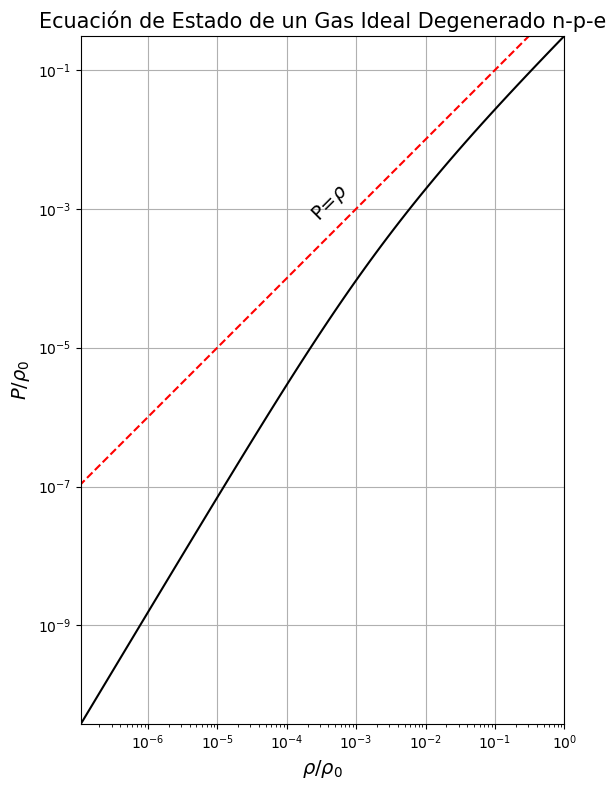
\includegraphics[width=0.55\linewidth]{Figuras/gas_npe}
	\caption[Ecuación de estado de gas ideal degenerado]{Ecuación de estado normalizada de un gas ideal degenerado de neutrones, protones y electrones. La ecuación de estado es causal ($c_s^2 = dP/d\rho < 1$).}
	\label{fig:eosnpe}
\end{figure}

Las integrales (\ref{eq:densidad_fermi_general}) y (\ref{eq:presion_fermi_general}) son analíticas, de modo que la ecuación de estado queda determinada por las expresiones $\rho(n_e)$ y $P(n_e)$ interpoladas sobre un rango de densidades relevante para estrellas de neutrones. El resultado de esta ecuación de estado se muestra en la figura \ref{fig:eosnpe}. Luego, empleando las ecuaciones TOV (\sistemaTOV) obtenemos las masas y radios de estrellas construidas con este material, como se muestra en la figura \ref{fig:mrnpe}. Este modelo sencillo predice una masa máxima de apenas 0.7$\masasol$, muy inferior a las masas que se han observado de estrellas de neutrones (listadas en la sección \ref{sec:obsNS}), motivando la búsqueda de modelos más realistas que logren replicar las observaciones.

\begin{figure}
	\centering
	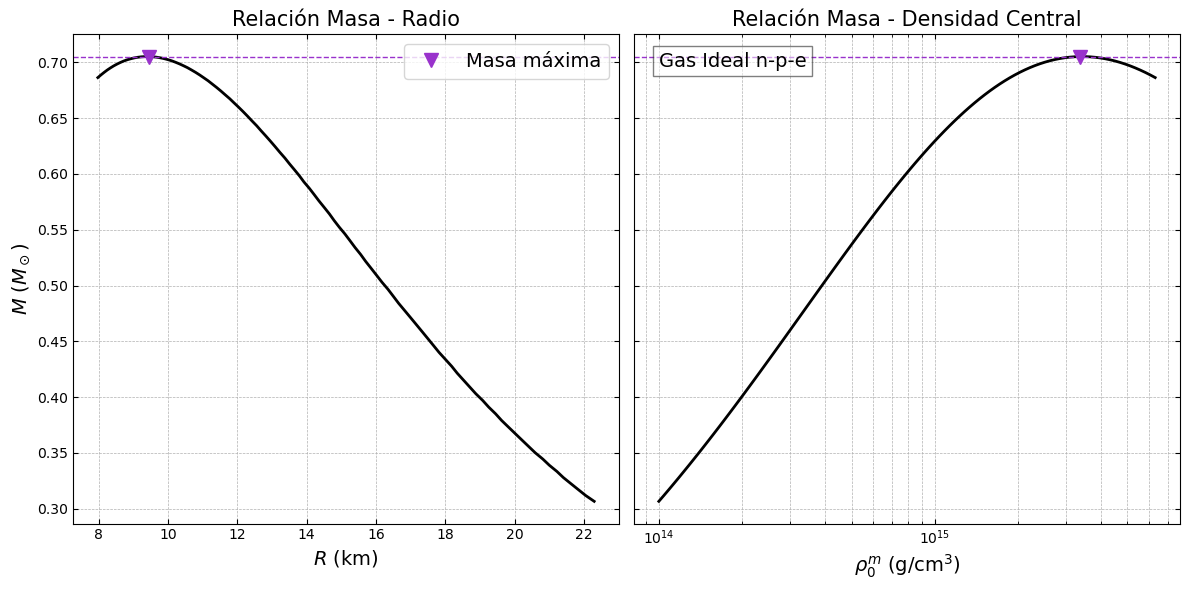
\includegraphics[width=0.9\linewidth]{Figuras/gas_npe_MR}
	\caption[Relaciones masa-radio de gas ideal degenerado]{Relaciones de masa - radio y masa - densidad central de masa de estrellas de neutrones constituidas por un gas ideal de neutrones, protones y electrones libres.}
	\label{fig:mrnpe}
\end{figure}



\section{Teoría Relativista de Campo Medio}
\label{sec:rmft}

La teoría relativista de campo medio es un marco teórico que describe las interacciones nucleares mediante el intercambio de mesones efectivos, extendiendo el modelo de gas degenerado (discutido en \ref{sec:gasnpe}) e incorporando naturalmente las características relativistas en condiciones de alta densidad. Formulada por Walecka en 1974 \cite{waleckaTheoryHighlyCondensed1974}, esta aproximación ofrece ventajas significativas respecto a enfoques no-relativistas basados en potenciales fenomenológicos, particularmente en su construcción covariante, su capacidad para reproducir simultáneamente las propiedades de saturación nuclear, el comportamiento asintótico a alta densidad, y la consistencia causal relativista. Adicionalmente, al ser una teoría efectiva, requiere de un menor esfuerzo computacional respecto a teorías más fundamentales como QCD.

El formalismo se construye a partir de un lagrangiano que describe nucleones interactuando a través de campos mesónicos. Los campos fermiónicos representan los grados de libertad nucleónicos y leptónicos, mientras que los campos bosónicos representan mesones que median las interacciones fuertes. La aproximación de campo medio consiste en reemplazar los operadores de campo mesónicos por sus valores esperados en el estado base degenerado:

\begin{equation}
	\langle \phi_i(x^\mu) \rangle = \phi_i^0 \equiv \text{constante},
	\label{eq:campo_medio}
\end{equation}

donde $\phi_i$ denota los diferentes campos mesónicos del modelo. Esta aproximación es válida cuando las fluctuaciones cuánticas son pequeñas comparadas con los valores esperados de los campos, condición que se satisface en materia nuclear densa cuanto mayor es la densidad del sistema \cite{waleckaRelativisticNuclearManyBody1986}.

\subsection{Simetrías y Conservaciones}

El formalismo de la teoría se construye sobre la teoría cuántica de campos. La densidad lagrangiana $\mathcal{L}(\psi, \partial_\mu \psi, \phi_a, \partial_\mu \phi_a)$ describe las interacciones entre campos fermiónicos $\psi$ y campos bosónicos $\phi_a$ junto con sus términos libres. Esta densidad lagrangiana debe satisfacer los requerimientos de localidad, covariancia de Lorentz, y las simetrías internas relevantes para las interacciones nucleares fuertes \cite{glendenningCompactStarsNuclear2000}. La acción del sistema se define como la integral de la densidad lagrangiana sobre el volumen espaciotemporal:

\begin{equation}
	S[\psi, \phi_a] = \int d^4x \, \mathcal{L}(\psi, \partial_\mu \psi, \phi_a, \partial_\mu \phi_a),
	\label{eq:accion}
\end{equation}

donde $d^4x$ es el elemento de volumen en coordenadas de Minkowski. El principio de acción estacionaria establece que las configuraciones físicas de los campos corresponden a los extremos de esta funcional, lo que conduce a las ecuaciones de movimiento mediante el cálculo variacional. Las ecuaciones de Euler-Lagrange para todos los campos son:

\begin{equation}
	\frac{\partial \mathcal{L}}{\partial \varphi_b} - \partial_\mu \left( \frac{\partial \mathcal{L}}{\partial (\partial_\mu \varphi_b)} \right) = 0,
	\label{eq:euler_lagrange}
\end{equation}

donde $\varphi_b$ representa todos los campos presentes. Estas ecuaciones se calculan para cada componente de los campos antes de aplicar la aproximación de campo medio, obteniendo el sistema de ecuaciones de movimiento a resolver. La teoría presenta simetrías externas e internas que determinan sus conservaciones y sus consecuencias físicas. Las simetrías externas son las transformaciones del grupo de Poincaré: traslaciones espaciotemporales $x^\mu \mapsto x'^\mu = x^\mu + a^\mu$ y boosts de Lorentz $x^\mu \mapsto x'^\mu = \Lambda^\mu{}_\nu x^\nu$. Las simetrías internas relevantes incluyen la simetría de gauge global $U(1)$ $\psi \mapsto e^{-i\lambda}\psi$ asociada con la conservación del número bariónico, y la simetría de isospín $SU(2)$ $\psi \mapsto e^{-i\boldsymbol{\tau}\cdot\boldsymbol{\lambda}}\psi$ asociada con la relación entre neutrones y protones, en la aproximación de iguales masas.

El teorema de Noether establece una correspondencia entre simetrías continuas del lagrangiano y cantidades conservadas. Para cada simetría continua existe una corriente conservada correspondiente que satisface una ecuación de continuidad. El tensor de energía-momento, asociado a la simetría externa, se define como:

\begin{equation}
	T^{\mu\nu} = \frac{\partial \mathcal{L}}{\partial (\partial_\mu \varphi_j)} \partial^\nu \varphi_j - \eta^{\mu\nu} \mathcal{L}, \quad \partial_\mu T^{\mu\nu} = 0,
	\label{eq:tensor_energia_momento}
\end{equation}

garantizando que la energía total $\int d^3x T^{00}$ del sistema se conserve en el tiempo en ausencia de fuerzas externas (flujos de momento en la frontera).

La corriente bariónica, asociada a la simetría interna $U(1)$, se define como:

\begin{equation}
	J_B^\mu = \sum_N \bar{\psi}_N \gamma^\mu \psi_N, \quad \partial_\mu J_B^\mu = 0,
	\label{eq:corriente_barionica}
\end{equation}

donde $\gamma^\mu$ son las matrices de Dirac y la suma se extiende sobre todas las especies de bariones presentes. Esto implica que el número bariónico $\int d^3x \, J_B^0$ integrado sobre el volumen total del sistema considerado permanece constante en el tiempo, reflejando el hecho experimental de que los bariones no se crean ni se destruyen en interacciones fuertes.

La corriente de isospín, asociada a la simetría interna $SU(2)$, se define como:

\begin{equation}
	\boldsymbol{J}_I^{\mu} = \sum_N \bar{\psi}_N \gamma^\mu \frac{\boldsymbol{\tau}}{2} \psi_N, \quad \partial_\mu J_I^{\mu a} = 0,
	\label{eq:corriente_isospin}
\end{equation}

donde $\boldsymbol{\tau} = \tau^a$ ($a = 1, 2, 3$) son las matrices de Pauli en el espacio de isospín. Aunque en la realidad física esta simetría está ligeramente rota por las diferencias de masa entre neutrones y protones (quarks up y down) y por las interacciones electromagnéticas, en aproximación se cumple. La conservación aproximada de isospín justifica el tratamiento unificado de neutrones y protones en modelos de materia nuclear.

Estas leyes de conservación derivadas del teorema de Noether añaden restricciones importantes sobre la dinámica del sistema y establecen conexiones directas entre las simetrías fundamentales de la teoría y las cantidades físicamente observables.


\section{Modelo del Estudio}

El modelo empleado en este trabajo incorpora nucleones (protones y neutrones) interactuando mediante campos mesónicos, y electrones libres. El lagrangiano total incluye términos para nucleones acoplados a los mesones, términos libres para electrones, un mesón escalar neutro $\sigma$ con autointeracciones no-lineales hasta cuarto orden, un mesón vectorial neutro $\omega^\mu$, y un mesón vectorial isovectorial $\boldsymbol{\rho^\mu}$ \cite{glendenningCompactStarsNuclear2000}:

\begin{equation}
	\begin{aligned}
		\mathcal{L} = &\bar{\psi} \left[ \gamma^\mu \left( i\partial_\mu - g_{\omega} \omega_\mu - \half g_{\rho} \boldsymbol{\tau} \cdot \rhomeson_\mu \right) - (m - g_{\sigma} \sigma) \right] \psi  \\
		&+ \frac{1}{2} \left( \partial_\mu \sigma \partial^\mu \sigma - m_\sigma^2 \sigma^2 \right) - \frac{1}{3}bm (g_\sigma\sigma)^3 - \frac{1}{4}c(g_\sigma\sigma)^4  \\
		&- \frac{1}{4} \omega_{\mu\nu} \omega^{\mu\nu} + \frac{1}{2} m_\omega^2 \omega_\mu \omega^\mu  \\
		&- \frac{1}{4} \rhomeson_{\mu\nu} \cdot \rhomeson^{\mu\nu} + \frac{1}{2} m_\rho^2 \rhomeson_\mu \cdot \rhomeson^\mu \\
		&- g_\rho \rhomeson_\mu \cdot [\rhomeson_\nu \cross \rhomeson^{\nu\mu} + 2g_\rho(\rhomeson^\mu \cross \rhomeson^\nu) \cross \rhomeson_\nu] \\
		&+ \bar{\psi}_e \left( i\gamma^\mu \partial_\mu - m_e \right) \psi_e,
		\label{eq:lagrangiano}
	\end{aligned}
\end{equation}

donde $\psi$ es una representación conveniente de los campos nucleónicos como un espinor de ocho componentes, $\psi_e$ es el campo del electrón, $\omega_{\mu\nu} = \partial_\mu \omega_\nu - \partial_\nu \omega_\mu$ y $\rhomeson_{\mu\nu} = \partial_\mu \rhomeson_\nu - \partial_\nu \rhomeson_\mu$ son los tensores antisimétricos de campo asociados a los mesones $\omega$ y $\rhomeson$ respectivamente, $m \approx 938.92 \text{MeV}$ es la masa de un nucleón considerada igual para protones y neutrones, y $m_i$ es la masa de la especie $i$. Los parámetros adimensionales de acoplamiento $g_{\sigma}$, $g_{\omega}$, $g_{\rho}$ cuantifican la intensidad de las interacciones nucleón-mesón, y los parámetros adimensionales $b$, $c$ regulan las autointeracciones del mesón sigma. En la construcción de este lagrangiano se acopla el campo escalar con la densidad escalar, el campo vectorial con la corriente bariónica, y el campo isovectorial con la 3-corriente de isospín. Esta última corriente contiene no solo una contribución por los nucleones, sino también una contribución por la corriente propia del campo $\rhomeson$ y otra por la interacción del mesón con su propia 3-corriente.

Las ecuaciones de movimiento para los campos se obtienen mediante las ecuaciones de Euler-Lagrange (\ref{eq:euler_lagrange}). Para los campos mesónicos, se satisfacen:

\begin{gather}
	\left(\square + m_\sigma^2\right) \sigma = g_\sigma\left[\bar{\psi} \psi - bm(g_\sigma\sigma)^2 - c(g_\sigma\sigma)^3\right], \label{eq:eom_sigma_full} \\
	(\square + m_\omega^2) \omega^\mu - \partial^\mu \partial_\nu \omega^\nu = g_{\omega} \bar{\psi} \gamma^\mu \psi, \label{eq:eom_omega_full} \\
	\begin{aligned}
		(\square + m_\rho^2) \rhomeson^\mu - \partial^\mu \partial_\nu \rhomeson^\nu = \half g_{\rho} \bar{\psi} \gamma^\mu \boldsymbol{\tau} \psi - 2g_\rho&[\rhomeson_\nu \cross \rhomeson^{\nu\mu} + \partial_\nu(\rhomeson^\mu \cross \rhomeson^\nu) \\ 
		&+ 4g_\rho[(\rhomeson^\mu \cdot \rhomeson_\nu)\rhomeson^\nu - (\rhomeson_\nu \cdot \rhomeson^\nu)\rhomeson^\mu]]. \label{eq:eom_rho_full}
	\end{aligned}
\end{gather}

Para los campos fermiónicos se obtienen las ecuaciones de Dirac, acoplada a los campos mesónicos para los nucleones y libre para los electrones:

\begin{gather*}
	\left[ \gamma^\mu \left( i\partial_\mu - g_{\omega} \omega_\mu - \half g_{\rho} \boldsymbol{\tau} \cdot \rhomeson_\mu \right) - (m - g_{\sigma} \sigma) \right] \psi = 0, \\
	(i\gamma^\mu \partial_\mu - m_e) \psi_e = 0.
\end{gather*}

Hasta el momento tenemos un conjunto de ecuaciones de movimiento diferenciales, no lineales y acopladas que describen la dinámica completa del sistema, cuya solución general es complicada. Para encontrar una solución sencilla empleamos la aproximación de campo medio descrita en la sección \ref{sec:rmft}, considerando que tenemos materia estática y uniforme en su estado base, de modo que los valores esperados de los campos mesónicos son constantes en el espacio y el tiempo. En este caso, las derivadas espaciales y temporales de los campos mesónicos se anulan, simplificando las ecuaciones de movimiento a un sistema algebraico acoplado. Mantendremos las etiquetas para los campos, recordado que ahora son el valor esperado en el estado base. Para los mesones (\ref{eq:eom_sigma_full} - \ref{eq:eom_rho_full}), sustituyendo consistentemente las fuentes de corriente por su valor esperado, se obtiene:

\begin{equation*}
	\begin{aligned}
		m_\sigma^2 \sigma &= g_\sigma \left[ \langle \bar{\psi} \psi \rangle - bm(g_\sigma\sigma)^2 - c(g_\sigma\sigma)^3\right], \\
		m_\omega^2 \omega^\mu &= g_{\omega} \langle \bar{\psi} \gamma^\mu \psi \rangle, \\
		m_\rho^2 \rhomeson^\mu &= \half g_{\rho} \langle \bar{\psi} \gamma^\mu \boldsymbol{\tau} \psi \rangle - 8g_\rho^2( (\rhomeson^\mu \cdot \rhomeson_\nu)\rhomeson^\nu - (\rhomeson_\nu \cdot \rhomeson^\nu)\rhomeson^\mu).
	\end{aligned}
\end{equation*}

Sin embargo, las primeras dos componentes del mesón $\rhomeson^\mu$ pueden escribirse en términos de los operadores de creación y aniquilación para mesones rho cargados $\rho_\pm^\mu = \frac{1}{\sqrt{2}}(\rho_1^\mu\pm i\rho_2^\mu)$, luego su valor esperado se anula en el estado base del sistema \cite{glendenningCompactStarsNuclear2000}, anulando el término fuente de la corriente propia del campo. Finalmente, el sistema de ecuaciones es:

\begin{equation}
	\begin{aligned}
		m_\sigma^2 \sigma &= g_\sigma \left[\langle \bar{\psi} \psi \rangle - bm(g_\sigma\sigma)^2 - c(g_\sigma\sigma)^3\right], \\
		m_\omega^2 \omega^\mu &= g_{\omega} \langle \bar{\psi} \gamma^\mu \psi \rangle = g_\omega \left[\langle \bar{\psi}_p \gamma^\mu \psi_p \rangle + \langle \bar{\psi}_n \gamma^\mu \psi_n \rangle \right], \\
		m_\rho^2 \rho_3^\mu &= \half g_{\rho} \langle \bar{\psi} \gamma^\mu \tau_3 \psi \rangle = g_\rho \left[\half \langle \bar{\psi}_p \gamma^\mu \psi_p \rangle - \half \langle \bar{\psi}_n \gamma^\mu \psi_n \rangle \right],
		\label{eq:eom_meson_mf}
	\end{aligned}
\end{equation}

notoriamente más sencillo luego de la aproximación. El siguiente paso para resolver los campos es hallar el valor esperado de las corrientes correspondientes a cada fuente de campo. Para los campos fermiónicos se tienen ecuaciones sin dependencia de las coordenadas de espaciotiempo, siendo estados propios de momento:

\begin{equation}
	\begin{gathered}
		\left[ \gamma^\mu \left( p_\mu - g_{\omega} \omega_\mu - g_{\rho} I_3 \rho_{3\mu} \right) - (m - g_{\sigma} \sigma) \right] \psi(p^\nu) = 0, \\
		(\gamma^\mu p_\mu - m_e) \psi_e(p^\nu) = 0,
		\label{eq:eom_fermion_mf}
	\end{gathered}
\end{equation}

donde $I_3 = \{+\half \; \text{para protones}, -\half \; \text{para neutrones}\}$ es el isospín de la partícula. En analogía con la ecuación de Dirac libre, definimos las cantidades de 4-momento y masa efectivas para nucleones:
%\vspace{-8pt}
\begin{equation}
	\begin{gathered}
		P^\mu = p^\mu - g_{\omega} \omega^\mu - g_{\rho} I_3 \rho_{3}^\mu,\\
		m^* = m - g_\sigma \sigma,
	\end{gathered}	
\end{equation}

obteniendo entonces la relación de dispersión relativista:

\begin{equation}
	\left(P_\mu P^\mu - m^{*2}\right)\psi(P^\nu) = 0,
\end{equation}

luego los valores propios de energía para los nucleones son:

\begin{equation}
	\epsilon(\Vec{p})_{I_3} = \sqrt{(\Vec{p}-g_\omega \Vec{\omega}-g_\rho I_3\Vec{\rho}_{3})^2+(m-g_\sigma\sigma)^2} + g_\omega\omega_0 + g_\rho I_3\rho_{30}.
	\label{eq:particleenergy} 
\end{equation}

Para calcular los valores esperados de las corrientes en (\ref{eq:eom_meson_mf}), usaremos un método económico para ahorrarnos la construcción de los campos fermiónicos. La forma general del valor esperado de un operador $\Gamma$ en el estado base de un sistema de muchos fermiones es:

\begin{equation}
	\langle \bar{\psi} \Gamma \psi \rangle = \sum_{\kappa}\int \frac{d^3p}{(2\pi)^3} (\bar{\psi} \Gamma \psi)_{\Vec{p},\kappa} \Theta(\epsilon_F - \epsilon(\Vec{p})_\kappa),
	\label{eq:valor_esperado_general}
\end{equation}

donde $\kappa$ representa los grados de libertad internos (espín, isospín), $\epsilon_F$ es la energía de Fermi del sistema cuya superficie $\epsilon(\Vec{p})=\epsilon_F$ no necesariamente es esférica, y la función escalón de Heaviside $\Theta(x) = \{1 \; \text{si} \; x > 0,\, 0 \; \text{si} \; x \leq 0\}$. $(\bar{\psi} \Gamma \psi)_{\Vec{p},\kappa}$ es el valor esperado, en el espacio de fase, del operador en el estado de un solo fermión con momento $\Vec{p}$ y grado de libertad interno $\kappa$. Para hallar el integrando acudimos al hamiltoniano de Dirac, y a su valor esperado, aislando $p^0$ de la ecuación para los nucleones (\ref{eq:eom_fermion_mf}):

\begin{equation}
	\begin{gathered}
		H_D^{I_3} = \gamma_0\left[\Vec{\gamma}\cdot\Vec{p} + \gamma^\mu(g_\omega \omega_\mu + g_\rho I_3\rho_{3\mu})+(m-g_\sigma\sigma)\right],\\
		(\psi^\dagger H_D^{I_3} \psi)_{\Vec{p},\kappa} = \epsilon(\Vec{p})_{\kappa} = P_0(\Vec{p}) + g_\omega\omega_0+g_\rho I_3\rho_{30}.
		\label{eq:hamiltonian}
	\end{gathered}
\end{equation}

Notamos que el hamiltoniano depende del isospín $I_3$ pero no del espín, de modo que los estados de espín son degenerados con ocupación dos. Tomando la derivada respecto a alguna variable $\xi$ del hamiltoniano (\ref{eq:hamiltonian}), y usando la regla de la cadena, obtenemos \cite{glendenningCompactStarsNuclear2000}:

\begin{equation}
	\begin{aligned}
		\frac{\partial}{\partial \xi} (\psi^\dagger H_D^{I_3} \psi)_{\Vec{p},\kappa} = (\psi^\dagger \frac{\partial H_D^{I_3}}{\partial \xi} \psi)_{\Vec{p},\kappa} + \epsilon(\Vec{p})_\kappa \cancel{\frac{\partial}{\partial \xi} (\psi^\dagger \psi)_{\Vec{p},\kappa}}, \\
	\end{aligned}
	\label{eq:derivada_hamiltoniano}
\end{equation}

donde el último término se anula porque $\psi$ es una función propia independiente. Tomando la derivada con respecto a $p^i$, se obtiene:

\begin{equation*}
	(\bar{\psi} \gamma^i \psi)_{\Vec{p},\kappa} = \frac{\partial \epsilon(\Vec{p})_\kappa}{\partial p^i},
\end{equation*}

y por la forma (\ref{eq:valor_esperado_general}), la corriente de nucleones es:

\begin{equation}
	\begin{aligned}
		\langle \bar{\psi} \gamma^i \psi \rangle &= 2\sum_{I_3}\int \frac{d^3p}{(2\pi)^3} \frac{\partial \epsilon(\Vec{p})_{I_3}}{\partial p^i} \Theta(\epsilon_F - \epsilon(\Vec{p})_{I_3}) \\
												 &= 2\sum_{I_3}\int \frac{d^2p}{(2\pi)^3} \int dp^i \frac{\partial \epsilon(\Vec{p})_{I_3}}{\partial p^i} \Theta(\epsilon_F - \epsilon(\Vec{p})_{I_3}) \\
												 &= 0,
		\label{eq:corriente_barionica_espacial}
	\end{aligned}		
\end{equation}

donde la integral se anula porque los valores de energía en las fronteras del volumen (de momento) son los mismos, luego la integral es una resta de números iguales. La componente espacial de la corriente bariónica es nula, como era de esperarse en un sistema estático y uniforme. Como las integrales para el protón y el neutrón son independientes, las componentes espaciales tanto del mesón $\omega$ como del mesón $\rho_3$ se anulan (ver ecuaciones (\ref{eq:eom_meson_mf})). Si tenemos solo componentes temporales de estos mesones, la energía de las partículas (\ref{eq:particleenergy}) depende únicamente de la magnitud del momento $\epsilon(\Vec{p}) = \epsilon(p)$, lo que implica que la superficie de Fermi es esférica en el espacio de momentos, simplificando la integral (\ref{eq:valor_esperado_general}). Ahora, tomando la derivada (\ref{eq:derivada_hamiltoniano}) con respecto a $\omega_0$:

\begin{equation*}
	(\bar{\psi} \gamma^0 \psi)_{\Vec{p},\kappa} = 1,
\end{equation*}

luego por (\ref{eq:valor_esperado_general}), la densidad bariónica es:

\begin{equation}
	\begin{aligned}
		\langle \bar{\psi} \gamma^0 \psi \rangle &= 2\sum_{I_3}\int \frac{4 \pi p^2 dp}{(2\pi)^3} \Theta(\epsilon_F - \epsilon(p)_{I_3}) \\
												 &= \int_0^{p_{Fp}} \frac{p^2 dp}{\pi^2} + \int_0^{p_{Fn}} \frac{p^2 dp}{\pi^2} \\
												 &= \frac{1}{3\pi^2}(p_{Fp}^3 + p_{Fn}^3) \equiv n_p + n_n = n_B,
		\label{eq:densidad_barionica}
	\end{aligned}
\end{equation}

donde $p_{Fp}$ y $p_{Fn}$ son los momentos de Fermi ($\epsilon_{FN} = \epsilon(p_{FN})_{I_3}$) para protones y neutrones respectivamente, y $n_B$ es la densidad bariónica total. De modo análogo, dado que el valor esperado es lineal y en vista de la ecuación para el campo rho (\ref{eq:eom_meson_mf}), la componente temporal de la tercera componente de la corriente de isospín es:

\begin{equation}
		\langle \bar{\psi} \gamma^0 \tau_3 \psi \rangle = \half (n_p - n_n) = n_3.
		\label{eq:densidad_isospin}
\end{equation}

Finalmente, tomando la derivada (\ref{eq:derivada_hamiltoniano}) con respecto a $m^*$:

\begin{equation*}
	(\bar{\psi} \psi)_{\Vec{p},\kappa} = \frac{m^*}{\sqrt{p^2 + m^{*2}}},
\end{equation*}

y por (\ref{eq:valor_esperado_general}), la densidad escalar es:

\begin{equation}
	\begin{aligned}
		\langle \bar{\psi} \psi \rangle &= 2\sum_{I_3}\int \frac{4 \pi p^2 dp}{(2\pi)^3} \frac{m^*}{\sqrt{p^2 + m^{*2}}} \Theta(\epsilon_F - \epsilon(p)_{I_3}) \\
										&= \sum_N \frac{1}{\pi^2}\int_0^{p_{FN}} \frac{p^2 (m-g_\sigma\sigma) dp}{\sqrt{p^2 + (m-g_\sigma\sigma)^{2}}} \equiv n_s. \\
		\label{eq:densidad_escalar}
	\end{aligned}
\end{equation}

Aunque todas las integrales anteriores son analíticas, la ecuación de movimiento para el campo escalar (\ref{eq:eom_meson_mf}) es una ecuación no lineal en $\sigma$ que debe resolverse autoconsistentemente con métodos numéricos. Además, resolviendo el sistema con $g_\sigma \sigma$, $g_\omega \omega_0$ y $g_\rho \rho_{30}$ como variables, el modelo tiene como parámetros libres unicamente los cocientes $g_\sigma/m_\sigma$, $g_\omega/m_\omega$ y $g_\rho/m_\rho$, junto con los parámetros de autointeracción escalar.

Para hallar la ecuación de estado recurrimos al valor esperado del tensor de energía-momento (\ref{eq:tensor_energia_momento}), al lagrangiano de la teoría (\ref{eq:lagrangiano}), la forma del tensor en este marco de referencia (\ref{eq:tensor_fluido_perfecto}) y al método descrito para encontrar valores esperados (\ref{eq:valor_esperado_general} - \ref{eq:derivada_hamiltoniano}). Luego, las expresiones para densidad de energía y presión son:

\begin{gather}
	\begin{aligned}
		\rho = \langle T^{00} \rangle &= \frac{1}{2}m_\sigma^2\sigma^2 + \frac{1}{3}bm(g_\sigma\sigma)^3 + \frac{1}{4}c(g_\sigma\sigma)^4 + \frac{1}{2}m_\omega^2\omega_0^2 + \frac{1}{2}m_\rho^2\rho_{30}^2 \\
		&+ \sum_N \frac{1}{\pi^2}\int_0^{p_{FN}} p^2 dp \sqrt{p^2 + (m-g_\sigma\sigma)^2} + \frac{1}{\pi^2}\int_0^{p_{Fe}} p^2 dp \sqrt{p^2 + m_e^2},
		\label{eq:densidad_energia}
	\end{aligned} \\
	\begin{aligned}
		P = \frac{1}{3}\sum_i \langle T^{ii} \rangle &= - \frac{1}{2}m_\sigma^2\sigma^2 - \frac{1}{3}bm(g_\sigma\sigma)^3 - \frac{1}{4}c(g_\sigma\sigma)^4 + \frac{1}{2}m_\omega^2\omega_0^2 + \frac{1}{2}m_\rho^2\rho_{30}^2 \\
		&+ \sum_N \frac{1}{3\pi^2}\int_0^{p_{FN}} \frac{p^4 dp}{\sqrt{p^2 + (m-g_\sigma\sigma)^2}} + \frac{1}{3\pi^2}\int_0^{p_{Fe}} \frac{p^4 dp}{\sqrt{p^2 + m_e^2}}.
		\label{eq:presion}
	\end{aligned}
\end{gather}

Estas expresiones son funciones de la densidad de número de protones, neutrones y electrones. Es necesario imponer condiciones adicionales para cerrar el sistema como en el caso del gas ideal de la sección \ref{sec:gasnpe}. Imponemos las mismas condiciones de neutralidad local de carga y equilibrio beta, obteniendo las ligaduras: 

\begin{gather}
	n_p = n_e \Rightarrow p_{Fp} = p_{Fe}, \\
	\epsilon(p_{Fn})_{I_3=-\half} = \epsilon(p_{Fp})_{I_3=+\half} + \epsilon_e(p_{Fe}), \label{eq:beta_equilibrio} \\
	p_{Fp} = (3\pi^2n_B - p_{Fn}^3)^{1/3},
\end{gather}

donde $\epsilon_e(p_{Fe}) = \sqrt{p_{Fe}^2 + m_e^2}$ es la energía de Fermi del electron y hemos definido el sistema como función de la densidad bariónica total $n_B$ mediante la conservación del número de bariones. Similar a la ecuación de campo escalar, la ecuación de equilibrio beta (\ref{eq:beta_equilibrio}) es una ecuación no lineal en $p_{Fn}$ que debe resolverse autoconsistentemente. Ahora que tenemos un sistema cerrado, podemos resolverlo numéricamente para cada valor de $n_B$, obteniendo la ecuación de estado $\rho(P)$ con métodos de interpolación, como se muestra en la figura \ref{fig:materiaestelarbase}. Sin embargo, aún es necesario determinar los cinco parámetros del modelo ($g_\sigma/m_\sigma$, $g_\omega/m_\omega$, $g_\rho/m_\rho$, $b$, $c$) para que el modelo sea físicamente consistente. Para ello, acudimos a las propiedades empíricas de la materia nuclear en saturación, descritas a continuación.

\begin{figure}[h]
	\centering
	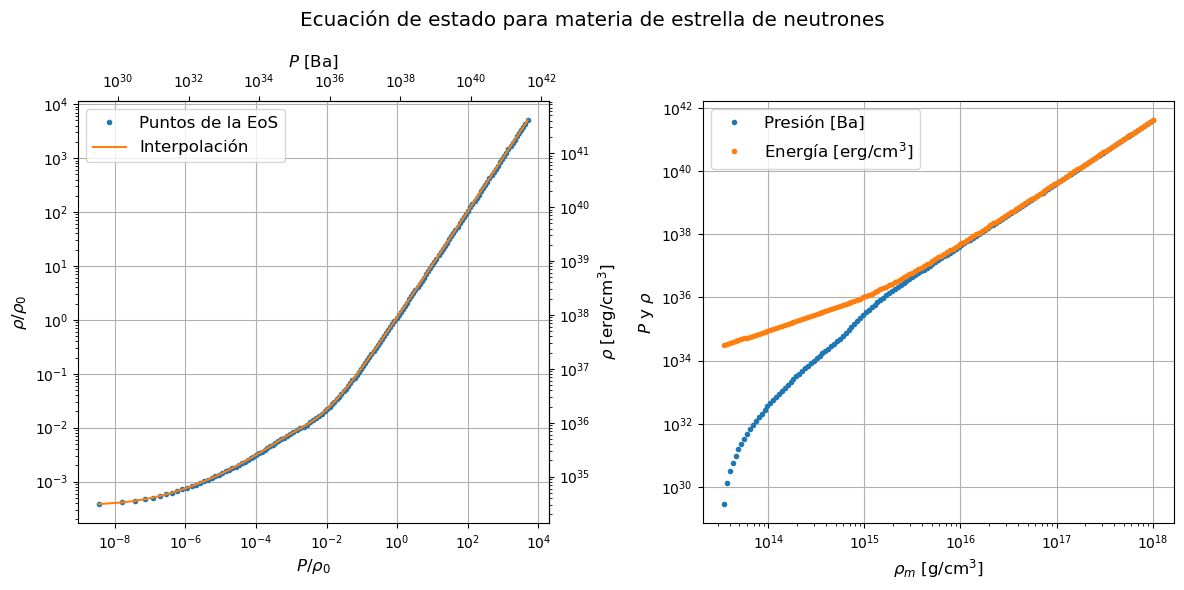
\includegraphics[width=0.95\linewidth]{Figuras/materia_estelar_base}
	\caption[Ecuación de estado para el núcleo de estrellas de neutrones.]{Ecuación de estado para el núcleo de estrellas de neutrones empleando teoría relativista de campo medio. Se usaron los parámetros $\left(\frac{g_\sigma}{m_\sigma}\right)^2=12.684\,\text{fm}^2$, $\left(\frac{g_\omega}{m_\omega}\right)^2=7.148\,\text{fm}^2$, $\left(\frac{g_\rho}{m_\rho}\right)^2=4.410\,\text{fm}^2$, $b=5.610\times10^{-3}$, $c=-6.986\times10^{-3}$.}
	\label{fig:materiaestelarbase}
\end{figure}


\subsection{Materia en Saturación Nuclear}

Si suprimimos los electrones libres del modelo (\ref{eq:lagrangiano}) y consideramos materia nuclear simétrica ($n_p = n_n$), el sistema se reduce a un fluido de nucleones interactuando mediante los campos mesónicos. Este sistema idealizado permite estudiar las propiedades de la materia nuclear en saturación, que corresponde a la densidad a la cual la materia nuclear alcanza su estado de mínima energía por nucleón. Mediante la materia a densidad de saturación es posible calibrar modelos microscópicos de la ecuación de estado nuclear pues tenemos mayor acceso experimental. Se caracteriza por cinco parámetros empíricos que añaden restricciones obligatorias para cualquier teoría microscópica válida \cite{kumarTheoreticalExperimentalConstraints2024}.

La densidad de saturación nuclear $n_0$ define la densidad a la cual la materia nuclear simétrica alcanza su estado de mínima energía de enlace por nucleón $\frac{B}{A}\big|_0  = \frac{\rho(n_0)}{n_0} - m$. Tras ajustar datos de 1654 núcleos en su estado base con N, Z $\geq 8$ a un modelo semi-empírico no relativista de gota líquida, se obtienen valores de $n_0 = 0.16114\, \text{fm}^{-3}$ y $\tfrac{B}{A}\big|_0 = -16.24\, \text{MeV}$, despreciando el término de superficie y el de Coulomb \cite{kumarTheoreticalExperimentalConstraints2024, myersNuclearPropertiesAccording1996}. En nuestro modelo (\ref{eq:lagrangiano}), estas propiedades de saturación se determinan numéricamente hallando el mínimo de la función $\tfrac{B}{A}(n_B)$ en ausencia de electrones, como se muestra de ejemplo en la figura \ref{fig:saturacionbase}.

\begin{figure}[h]
	\centering
	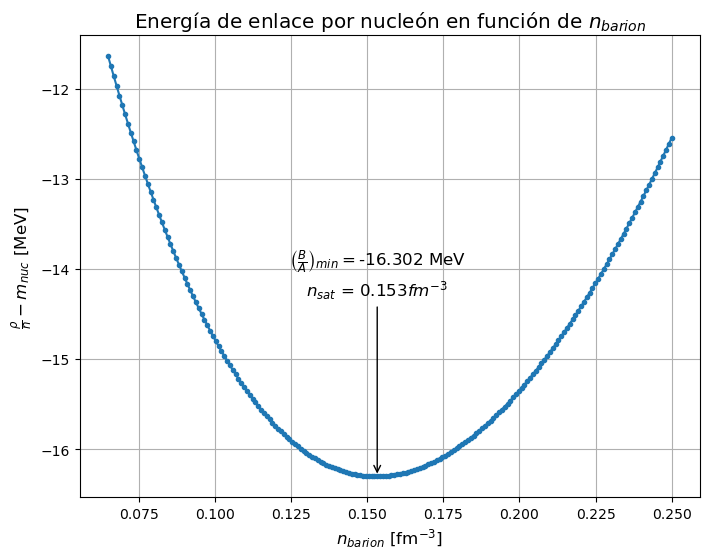
\includegraphics[width=0.7\linewidth]{Figuras/saturacion_base}
	\caption[Energía de enlace por nucleón en saturación nuclear]{Energía de enlace por nucleón en función de la densidad bariónica para materia nuclear simétrica sin electrones. La densidad de saturación $n_0$ y la energía de enlace por nucleón en saturación $\frac{B}{A}\big|_0$ se señalan en el mínimo. Se usaron los parámetros $\left(\frac{g_\sigma}{m_\sigma}\right)^2=12.684\,\text{fm}^2$, $\left(\frac{g_\omega}{m_\omega}\right)^2=7.148\,\text{fm}^2$, $\left(\frac{g_\rho}{m_\rho}\right)^2=4.410\,\text{fm}^2$, $b=5.610\times10^{-3}$, $c=-6.986\times10^{-3}$.}
	\label{fig:saturacionbase}
\end{figure}

El módulo de compresibilidad nuclear $K_0$ caracteriza la rigidez de la materia nuclear ante compresiones alrededor del punto de saturación:

\begin{equation*}
	K_0 = 9n_0^2 \frac{\partial^2}{\partial n^2}\left(\frac{\rho}{n}\right)\bigg|_{n=n_0}.
\end{equation*}

Este parámetro es determinante para la extrapolación de la ecuación de estado a densidades supranucleares, y es estimado mediate las resonancias monopolares en núcleos pesados. Considerando un modelo de cadena de núcleos para esta resonancia en $^{208}$Pb, se obtiene $K_0 = 230 \pm 40$ MeV \cite{kumarTheoreticalExperimentalConstraints2024, khanConstrainingNuclearEquation2012}. Esta cantidad está relacionada algebraicamente con cantidades del modelo con materia simétrica en saturación:

\begin{equation}
	\begin{gathered}
		K_0 = \frac{6}{\pi^2}A_\omega p_F^3 + \frac{3p_F^2}{\sqrt{p_F^2 + (m-x_\sigma)^2}} - \frac{6A_\sigma}{\pi^2}\frac{p_F^3(m-x_\sigma)^2}{p_F^2+(m-x_\sigma)^2}F^{-1}, \\
		F = 1 + A_\sigma x_\sigma[2bm+3cx_\sigma]+\frac{2A_\sigma}{\pi^2}\int_0^{p_F} \frac{p^4 dp}{(p^2+(m-x_\sigma)^2)^{3/2}},
	\end{gathered}
	\label{eq:modulo_compresibilidad}
\end{equation}

donde $A_i = (g_i/m_i)^2$ y $x_\sigma = g_\sigma \sigma$. 

La energía de simetría $a_\text{sym}$ cuantifica el costo energético de desviarse de la composición simétrica. Se define como:

\begin{equation*}
	a_\text{sym} = \frac{1}{2} \frac{\partial^2}{\partial t^2}\left(\frac{E}{A}\right)\bigg|_{t=0},
\end{equation*}

donde $t = (n_n - n_p)/n_B$ es el parámetro de asimetría de isospín. La pendiente de la energía de simetría $L_0$ describe la dependencia con la densidad de la energía de simetría alrededor de la densidad de saturación:

\begin{equation*}
	L_0 = 3n_0 \frac{\partial a_\text{sym}}{\partial n}\bigg|_{n=n_0},
\end{equation*}

y estas dos cantidades, tras una revisión de 28 estimaciones de experimentos tanto terrestres como de observaciones astronómicas de estrellas de neutrones, se estiman valores representativos de $a_\text{sym} = 31.6 \pm 2.7$ MeV y $L_0 = 58.9 \pm 16$ MeV \cite{kumarTheoreticalExperimentalConstraints2024, liUnderstandingAstrophysicalEffects2019}. Es de notar que, si bien el valor fiducial tiene una baja incertidumbre, las estimaciones individuales de $L_0$ varían ampliamente, con intervalos de confianza que oscilan entre 20 y 120 MeV debido a la dificultad para acceder a materia altamente asimétrica en el laboratorio. En nuestro modelo, estas cantidades pueden calcularse como:
\vspace{-6pt}
\begin{align}
	a_\text{sym} &= \frac{p_F^2}{6\sqrt{p_F^2 + (m-x_\sigma)^2}} + \frac{1}{8}A_\rho n_B, \label{eq:energia_simetria} \\
	L_0 &= \frac{p_F^2}{3\sqrt{p_F^2 + (m-x_\sigma)^2}}\left(1 - \frac{p_F^2}{p_F^2 + (m-x_\sigma)^2}\right) + \frac{3}{8}A_\rho n_B. \label{eq:pendiente_simetria}
\end{align}

Estas cinco propiedades empíricas ($n_0$, $\frac{B}{A}\big|_0$, $K_0$, $a_\text{sym}$, $L_0$) definen restricciones que cualquier ecuación de estado microscópica debe satisfacer para ser físicamente viable. En el contexto de la teoría relativista de campo medio, estas propiedades y sus incertidumbres se utilizan para determinar el espacio de parámetros del modelo físicamente aceptable.

\subsection{Corteza de la estrella}

El modelo de teoría relativista de campo medio desarrollado es una descripción de la materia nuclear en el régimen de alta densidad, específicamente para densidades bariónicas superiores a aproximadamente $0.1$ fm$^{-3}$ o $\rho_m \gtrsim 1.7 \times 10^{14}$ g/cm$^3$, donde las interacciones nucleón-nucleón dominan la dinámica del sistema y la aproximación de campo medio tiene sentido. Sin embargo, las estrellas de neutrones presentan una estructura estratificada que incluye regiones de menor densidad donde esta aproximación deja de ser aplicable. La corteza de la estrella, que se extiende desde la superficie hasta el núcleo denso, abarca un rango de densidades de varios órdenes de magnitud y requiere tratamientos teóricos distintos según el régimen de densidad considerado \cite{shapiroBlackHolesWhite2008}.

Para densidades inferiores al punto de goteo de neutrones ($n_{\text{drip}} \approx 2.4\times10^{-4}$ fm$^{-3}$ o $\rho \approx 4 \times 10^{11}$ g/cm$^3$), la materia se compone de una red cristalina de núcleos pesados embebidos en un gas degenerado de electrones, configuración conocida como corteza externa. En este régimen, la ecuación de estado BPS (Baym, Pethick y Sutherland, 1971) \cite{baymGroundStateMatter1971} describe consistentemente con base en la minimización de la energía del estado base de núcleos atómicos para cada densidad, junto con la contribución del gas de electrones relativista. El modelo BPS determina la composición nuclear óptima mediante la competencia entre la energía de masa nuclear, la energía de Coulomb de la red, y la presión del gas electrónico. Por encima de la densidad de goteo de neutrones y hasta densidades del orden de $0.2$ fm$^{-3}$ o $\rho \approx 3.2 \times 10^{14}$ g/cm$^3$ se encuentra la corteza interna, donde los núcleos coexisten con un gas de neutrones libres además del gas de electrones. En este régimen, la ecuación de estado BBP (Baym, Bethe y Pethick, 1971) \cite{baymNeutronStarMatter1971} describe la materia mediante un modelo de gota líquida que considera las contribuciones energéticas de los núcleos, el gas de neutrones libres, y las interacciones nucleares efectivas de la red. Este modelo determina autoconsistentemente la composición nuclear y la fracción de neutrones libres mediante la minimización de la energía total del sistema, que incluye términos de energía de superficie, energía de Coulomb, y energía de simetría nuclear.

El alcance del presente estudio se concentra en la descripción microscópica de la materia nuclear en el régimen de altas energías en las estrellas de neutrones, donde las densidades superan varias veces la densidad de saturación $n_0$, justificando el uso de la teoría relativista de campo medio. Por esta razón, utilizamos las ecuaciones de estado estándar BPS y BBP como entrada externa para integrar las ecuaciones de estructura en las regiones de baja densidad, sin profundizar en los detalles microscópicos de su construcción fuera del marco de este trabajo.

Para construir una ecuación de estado unificada que abarque todo el rango de densidades presente en la estrella, desde la superficie hasta el núcleo, empleamos el método de interpolación \href{https://es.wikipedia.org/wiki/Interpolador_c\%C3\%BAbico_de_Hermite}{PCHIP} (Piecewise Cubic Hermite Interpolating Polynomial), que garantiza una transición suave y monótona entre las diferentes ecuaciones de estado. Este método de interpolación preserva la forma de los datos y evita oscilaciones no físicas que podrían introducir otros métodos de interpolación polinómica. Definimos la densidad de empalme entre la ecuación de estado BBP y nuestro modelo de teoría relativista de campo medio en $n_B = 0.062$ fm$^{-3}$, correspondiente a una densidad de masa de aproximadamente $1.04 \times 10^{14}$ g/cm$^3$. Esta elección se fundamenta en la necesidad de garantizar la causalidad del fluido en toda la estrella, es decir, que la velocidad del sonido $c^2_s = dP/d\rho$ no exceda la velocidad de la luz $c$ en ningún punto. El resultado de esta interpolación para un conjunto de parámetros de ejemplo y su comprobación de causalidad se muestra en la figura \ref{fig:causalidadmateriabase}.

\begin{figure}[h]
	\centering
	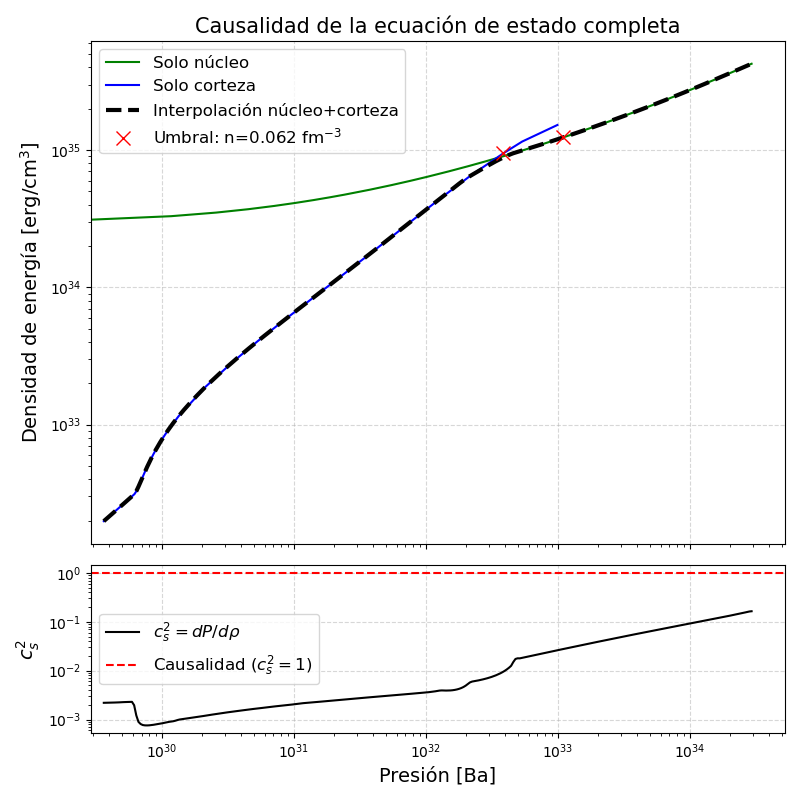
\includegraphics[width=0.7\linewidth]{Figuras/causalidad_materia_estelar_completa}
	\caption[Ecuación de estado unificada y causalidad.]{Ecuación de estado unificada para la estrella de neutrones, construida mediante interpolación PCHIP entre las ecuaciones de estado BPS, BBP y el modelo RMFT. El panel inferior muestra el cuadrado de la velocidad del sonido $c_s^2$ para verificar la condición de causalidad. Se usaron los parámetros $\left(\frac{g_\sigma}{m_\sigma}\right)^2=12.684\,\text{fm}^2$, $\left(\frac{g_\omega}{m_\omega}\right)^2=7.148\,\text{fm}^2$, $\left(\frac{g_\rho}{m_\rho}\right)^2=4.410\,\text{fm}^2$, $b=5.610\times10^{-3}$, $c=-6.986\times10^{-3}$.}
	\label{fig:causalidadmateriabase}
\end{figure}

% Figura: Interpolación PCHIP
% [Espacio para figura mostrando P vs rho para BPS, BBP, interpolación PCHIP, y modelo RMFT, 
% con énfasis en la región de empalme en n_B = 0.062 fm^{-3}. Incluir panel secundario 
% mostrando la velocidad del sonido v_s/c para verificar causalidad (v_s < c) en toda la región.]


%Capítulo 4
\chapter{Resultados y discusión}
\thispagestyle{fancy}

% Resultados
\section{Dependencia de los parámetros en la propiedades}

\section{Masa maxima con las propiedades (parametros)}



%Capítulo 5
\chapter{Conclusiones}
\thispagestyle{fancy}

% Conclusiones

\section{Principales hallazgos}

\section{Limitaciones del estudio}

\section{Recomendaciones para futuros trabajos}

%Capítulo 6
\chapter{Apéndices}
\thispagestyle{fancy}

% Anexos

% Agregar consentimiento informado usado, códigos?


%\bibliographystyle{ieeetr}
%\bibliography{PropuestadeTesis}
\printbibliography


%\renewcommand{\bibname}{Referencias}
%\addcontentsline{toc}{chapter}{Referencias}
%\bibliography{Bibliografia} % Reemplaza 'biblio' con el nombre de tu archivo .bib
\end{document}
